\section{\textit{Application to Process and Produce Analytic Data (APPA)}}

Definir uma boa base de dados é o ponto mais critico durante a criação de uma inteligência supervisionada. O \textit{Application to Process and Produce Analytic Data} (APPA), ou, Aplicação para Processamento e Produção de Dados Analíticos, é um ferramenta criada pelo autor dessa pesquisa capaz de cadastrar tarefas, em qualquer linguagem e utilizar delas para coletar e processar esses dados afim de gerar uma base de conhecimento.

Explicando com mais detalhes, a Figura \ref{fig:appa_eng} mostra o funcionamento da ferramenta. Existe uma arquivo chamado \textit{config.yml} que tem mapeado todas as tarefas e entidades de processamento. Essas tarefas podem ser escritas em qualquer linguagem de programação e algumas delas podem ser responsáveis por coletar dados, os scripts que são escritos com intuito de retornar dados para processamento são chamados coletores.

\begin{figure}
    \centering
    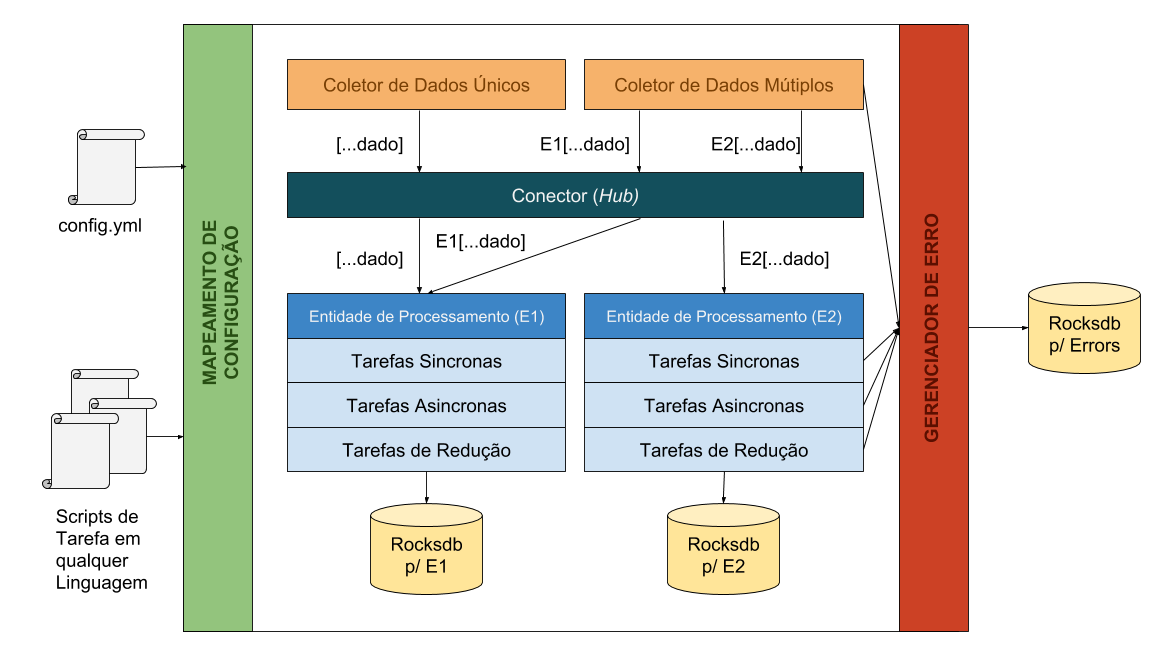
\includegraphics[width=.8\textwidth]{imagens/appa_eng.png}
    \caption{Diagrama demonstrando o funcionamento da ferramenta APPA}
    \label{fig:appa_eng}
\end{figure}

Um dado emitido por um coletor é marcado ou não por uma \textit{tag}, ou marcação, essa responsável por creditar qual coletor será responsável por processar. Por padrão um dado enviado sem destino é marcado com o simbolo \textit{underline}. Toda tarefa dentro do APPA é considerada uma tarefa com múltiplas saídas, logo, é possível enviar dados em lotes e tempo real para que o APPA processe dentro das entidades. 

Entidades de processamento, por sua vez, são compostas por coletores e tarefas de processamento. As tarefas de processamento podem ser síncronas ou assíncronas, ambas executam individualmente por unidade de dado, algo similar a uma linha de dados de um banco, a diferença é seu formato de execução, como o próprio nome fala as tarefas assíncronas não respeitam ordem de execução e são executadas paralelamente pelo processador. Alem disso existem as redutoras e/ou mapeadoras, que consumirão todo o banco gerado após a execução das tarefas síncronas e assíncronas e retornara um novo estado para o banco total. Cada entidade gera seus dados em um banco incorporado isolado para os dados processados por elas.

Diferente de outras ferramentas, o processo de mineração nunca é interrompido. Qualquer erro que aconteça na aplicação é gerenciado por uma camada e registrado em um banco de erros, após isso o processamento segue para os demais dados.
